% #region PREAMBEL OG PAKKER
\documentclass[a4paper, 12pt]{article}  % DOKUMENTKLASSE
\title{Eksamen ØKO1001\\Del 2: Økonomi} % TITTEL
\author{Kandidatnr. 10026}              % FORFATTER
\date{\today}                           % DATO & FAG

\usepackage[english, norsk]{babel}      % NORSK SPRÅK
\usepackage[                            % BIBLIOGRAFI
    backend=biber,
    style=apa,
    ]{biblatex}
\usepackage{csquotes}                   % PAKKE TIL BABEL
\addbibresource{ref.bib}                % PATH TIL BIBLIOGRAFI
\usepackage[hidelinks]{hyperref}        % LENKER I TOC OG GENERELT
\usepackage[margin=1in]{geometry}       % VANLIG STØRRELSE MARGIN
\setlength{\parindent}{0em}             % SKILLER AVSNITT
\setlength{\parskip}{1em}               % SKILLER AVSNITT
\usepackage{setspace}
\setstretch{1.4}                        % 1.5 LINJEAVSTAND
\usepackage{graphicx}                   % BILDER \includegraphics[OPTIONS]{PATH}
\usepackage{kantlipsum}                 % FYLLTEKST I KANT-STIL (kant[n-m])
\usepackage{amsfonts}                   % BLACKBOARD BOLD FONT (\mathbb{N})
\usepackage{import}                     % IMPORTER FILER (\import{PATH}{FILE})
\usepackage{caption}                    % PAKKE FOR BEDRE CAPTIONS I FIGURER
\usepackage{float}                      % FLYTT FIGURER 
\usepackage{booktabs, multirow} % for borders and merged ranges
\usepackage{soul}% for underlines
\usepackage[table]{xcolor} % for cell colors
\usepackage{changepage,threeparttable} % for wide tables
\usepackage[shortlabels]{enumitem}
% #endregion
\begin{document}
% #region INNHOLDSFORTEGNELSE
\maketitle
\vfill
\begin{center}
  ØKO1001 - Ledelse
\end{center}
\thispagestyle{empty}
\addtocounter{page}{-1}
\newpage
% \tableofcontents % INNHOLDSFORTEGNELSE
% \thispagestyle{empty}
% \addtocounter{page}{-1}
% \newpage
% #endregion
\section*{Oppgave 1}

\begin{enumerate}[(a)]
  \item Dette spørsmålet kan vurderes fra flere synspunkt ut i fra hvilket ståsted man har. Ønsker man høyest mulig inntekt vil prisen bli det den kunden som er villig til å betale mest, kan betale. Det bedriftsøkonomiske synspunktet blir besvart i neste deloppgave. Hvis jeg skal vurdere spørsmålet ordrett slik det er stilt og vurdere min personlige mening, ville jeg nok gitt bort notatene gratis.

  \item Hvis man ser på det bedriftsøkonomisk kostet det å skrive notatene \(20 \times 600\textrm{kr} = 12000\textrm{kr}\), 
  sammenliknet med alternativet å jobbe 20 timer. Antatt at målet er å i det minste gå i null, ønsker man å tjene opp igjen disse pengene ved et salg. 
  Den laveste prisen per notat vil da være 1200kr delt på antall kunder man vet er villig til å kjøpe.  
  Oppgaven oppga ikke et antall kunder, og nevnte kun at ``mange vil kjøpe''. 
  
  Eksempel hvis ``mange'' = 20: \(12000\textrm{kr} \div 20 = 600\textrm{kr}\)

  Dette er med en antagelse at man kan selge flere kopier av notatene,
  hvis bare en kopi kan selges blir prisen 12000kr.

  \item I oppgave (a) kan det være viktig å trekke inn alternativkostnaden til notatene, som indikerer at den reelle kostnaden av å skrive de var de 12000kr man unngikk å tjene ved å jobbe. Dette betyr da at hvis man vurderer å gi bort notatene gratis, har man reelt tapt 12000kr.
\end{enumerate}

\newpage
\section*{Oppgave 2}
\begin{enumerate}[(a)]
  \item Beregnet utsalgspris eks. MVA blir 15,68kr om man ønsker en fortjenesteprosent på 33.33\%. Se utregning under:
  \begin{figure}[H]
    \centering
    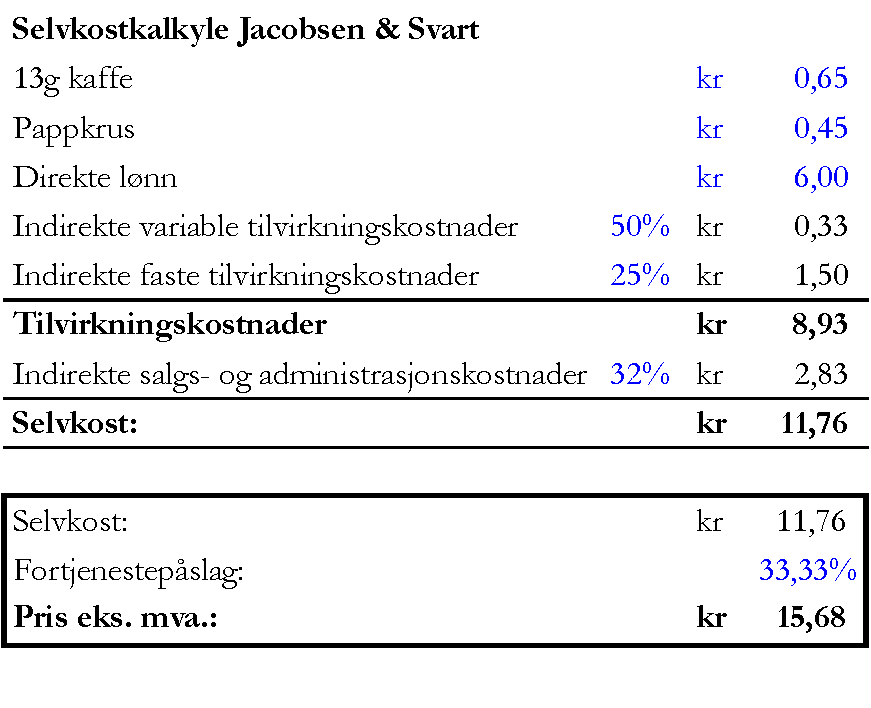
\includegraphics[width=12cm]{img/selvkostkalkyle.pdf}
  \end{figure}

  \item Økonomisk vil Jacobsen \& Svart tape totalt 413,80kr, eller 2,76kr per kopp, hvis de aksepterer ordren. Med oppgavens antagelse om at ordren ikke vil gi noen positive eller negative ringvirkninger, er derfor ikke en god økonomisk beslutting.
  \begin{figure}[H]
    \centering
    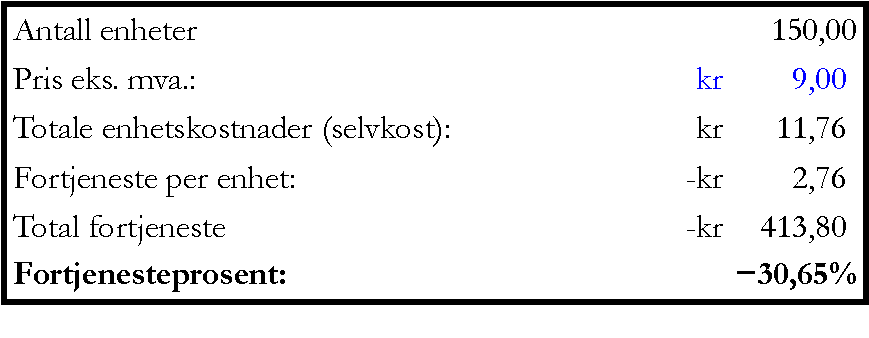
\includegraphics[width=12cm]{img/selvkostkalkyle2.pdf}
  \end{figure}
\end{enumerate}

\newpage
\section*{Oppgave 3}

Under følger punkter/tema/spørsmål jeg ville tatt opp om jeg skulle gjøre en analyse av Gønne på AS sine regnskapstall. Påstandene jeg kommer med er gjort i antagelse av hva tallene kan bety i sammenhengen de forekommer. Men å lese tall uten riktig kontekst kan være farlig, fordi som vi vet:

\begin{displayquote}
\emph{Tallene taler aldri for seg selv.}
 -- \parencite{berg19}
\end{displayquote}

\begin{itemize}
  \item Ordinære avskrivninger økte med ca. 30\% i 2019 og ca. 18,5\% i 2020. Vanlig vis holdes denne konstant, og må passe på å ikke fortsette økningen i like stor grad.
  
  \item Lønnskostnadene i 2020 stupte kraftig. Hva var grunnen til det? Permittering av ansatte pga. pandemien? Inntektene og kostnadene tilsier ikke at det skulle være nødvendig.
  
  \item Kundefordring økte kraftig i 2020. Dette kan være et tegn på at det selges til kunder en elles ikke har, eller at eksisterende kunder utsetter betalinger. Det kan være lurt å foreta en oversikt over kundenes gjennomsnittlige forfall. 
  
  \item Omløpsmidlene i bank har sunket betydelig de siste to årene. Summen av omløpsmidlene er fortsatt god, så lenge man har oversikt over de nevnte kundefordringene. Men det kan være lurt å ikke plassere alle eggene i én kurv.
  
  \item Den kortsiktige gjelden har hatt en fallende utvikling siden 2017, men steg kraftig i 2020. Høy kortsiktig gjeld kan skade bedriftens likviditet på sikt, og gjøre at bedriften er dårligere rustet i nedgangstider.
  
  \item Bedriftens likviditet har reelt økt siden 2019 og er på sitt høyeste ut i fra tilgjengelige tall. Den totale kortsiktige gjelden og de totale omløpsmidlene har tendert med hverandre de siste fire årene, men omløpsmidlene har hatt de største reelle endringene, både opp og ned.
  \begin{figure}[H]
    \centering
    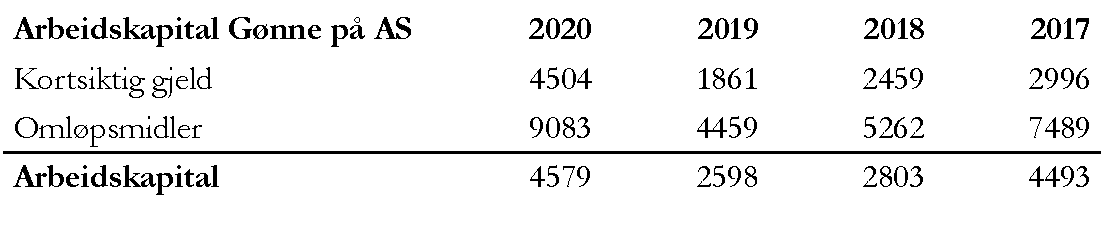
\includegraphics[width=14cm]{img/likviditet.pdf}
  \end{figure}
\end{itemize}

\newpage
\printbibliography[heading=bibintoc] % LAGER BIBLIOGRAFI

\end{document}
